\section{Conclusion}
\begin{comment}
By continuously generating new forecasts and scrutinizing the residuals, which represent the disparities between forecasted and actual values, provides valuable real-time insights into the system's dynamic behavior. This iterative forecasting approach enables a proactive response to anomalies, allowing for timely adjustments to maintain system stability and performance.

In a scenario where the actual temperature experiences an abrupt increase, deviations between the forecasts and actual values become pronounced, resulting in elevated residuals. It is essential to recognize that this deviation is a notable anomaly, indicative of a significant shift in the system. Comparing this to a prior anomaly, a substantial temperature drop, reveals interesting dynamics. The contextualization of anomalies is crucial; the second temperature drop, while less drastic in residuals, gains significance when considered in conjunction with the first anomaly.

Furthermore, the first anomaly, marked by a transient increase in residuals, emphasizes the system's adaptability to new input data. The swift decline in residuals following the initial anomaly showcases the forecasting system's responsiveness and its ability to quickly recalibrate to changing conditions. This responsiveness is a key characteristic, indicating that sustained spikes in residuals over extended periods would be atypical and may warrant closer investigation. In summary, the analysis of residuals not only aids in anomaly detection but also provides insights into the system's adaptability and responsiveness to evolving conditions.
\end{comment}
Continuously making new predictions and carefully examining the differences between these predictions and the actual values provides us with real-time insights into how a system behaves. This iterative forecasting approach helps us respond proactively to anomalies, making timely adjustments to keep the system stable and performing well.

For instance, if the actual temperature suddenly increases, the differences between our predictions and the actual values become more noticeable, leading to higher differences called residuals. Recognizing this difference is crucial because it indicates a significant shift in the system. Comparing this event to a previous anomaly, such as a substantial temperature drop, reveals interesting patterns. Contextualizing these anomalies is important; even if the second temperature drop has smaller residuals, it gains significance when considered with the first anomaly.

Moreover, the first anomaly, marked by a temporary increase in residuals, highlights the system's ability to adapt to new input data. The quick decrease in residuals after the initial anomaly shows that the forecasting system is responsive and can rapidly adjust to changing conditions. This responsiveness is a key feature, suggesting that prolonged increases in residuals would be unusual and might need closer investigation. In summary, analyzing residuals not only helps detect anomalies but also provides insights into the system's adaptability and responsiveness to changing conditions.

\clearpage 


\section {Recommendations}

Temperature and current serve as initial indicators of deterioration in electric motors, often signaling an underlying fault in most cases. However, for precise fault pinpointing, a comprehensive set of parameters must be collected. Beyond temperature and current, additional parameters play a pivotal role in a thorough fault analysis. These include:

\begin{itemize}
    \item \textbf{Motor Phase Change:}
    Monitoring changes in motor phases provides crucial insights into the system's electrical health. Discrepancies or irregularities in phase characteristics can signify potential faults or imbalances.

    \item \textbf{Shaft Vibrations:}
    Vibrations in the motor shaft offer valuable information regarding mechanical integrity. Anomalies in vibrations can point to issues such as misalignments, imbalances, or mechanical wear, contributing to a holistic understanding of the motor's condition.

    \item \textbf{Shaft Imbalance:}
    Detecting imbalances in the motor shaft is critical for maintaining smooth operation. Imbalances can result in undue stress on components, leading to accelerated wear and potential system failures if left unaddressed.

    \item \textbf{Shaft Misalignment:}
    Monitoring shaft alignment is vital as misalignments can cause significant damage over time. Misalignments may lead to increased friction, heat, and wear, impacting the overall efficiency and lifespan of the electric motor.
\end{itemize}

By incorporating these additional parameters into the monitoring and analysis process, it becomes possible to enhance the diagnostic capabilities and address potential faults proactively. The multi-parameter approach ensures a more comprehensive understanding of the motor's health, enabling timely interventions to prevent or mitigate issues before they escalate.
alignment. Misalignments may lead to increased friction, heat, and wear, impacting the overall efficiency and lifespan of the electric motor.
\pagebreak


\section{Project Budget}
\setlength{\arrayrulewidth}{0.5mm}
\setlength{\tabcolsep}{18pt}
\renewcommand{\arraystretch}{1.5}
\begin{tabular}{ |p{2.5cm}|p{3.5cm}|p{2.5cm}|p{2.5cm}|  }
	\hline
	\multicolumn{4}{|c|}{\textbf{Item List}} \\
	\hline
	ITEM & SPECIFICATION & QUANTITY & PRICE \\
	\hline
	Esp32 & 32s, usb 2.0 Cable Type A/B & 1 & 4500 \\
	\hline
	Therm Amplifier & MAX31855K & 1 & 790 \\
	\hline
	Dev Board & NodeMCU 32S ESP32/ CH340c  & 1 & 1700\\
	\hline
	Thermocouple K type&Temp range: 0-600  & 1 & 1450\\
	\hline
	Thermocouple DH22 & 3.3-6v input  & 1 & 500\\
	\hline
	Power Unit & 12v/5W SMPS Module & 1   & 1700\\
	\hline
	Breadboard & MB102  165*55*50mm & 2 & 200\\
	\hline
	Jumper Wires & 20cm male 20cm female & 80 & 500 \\
	\hline
	% Vibration accelerometer & Piezoelectric 308 m175 308175 & 1 & 6500 \\
	% \hline
	\textbf{Total} & & &7790 \\
	\hline
\end{tabular}



% \section{Work Plan}
% \begin{figure}[!h]
% 	%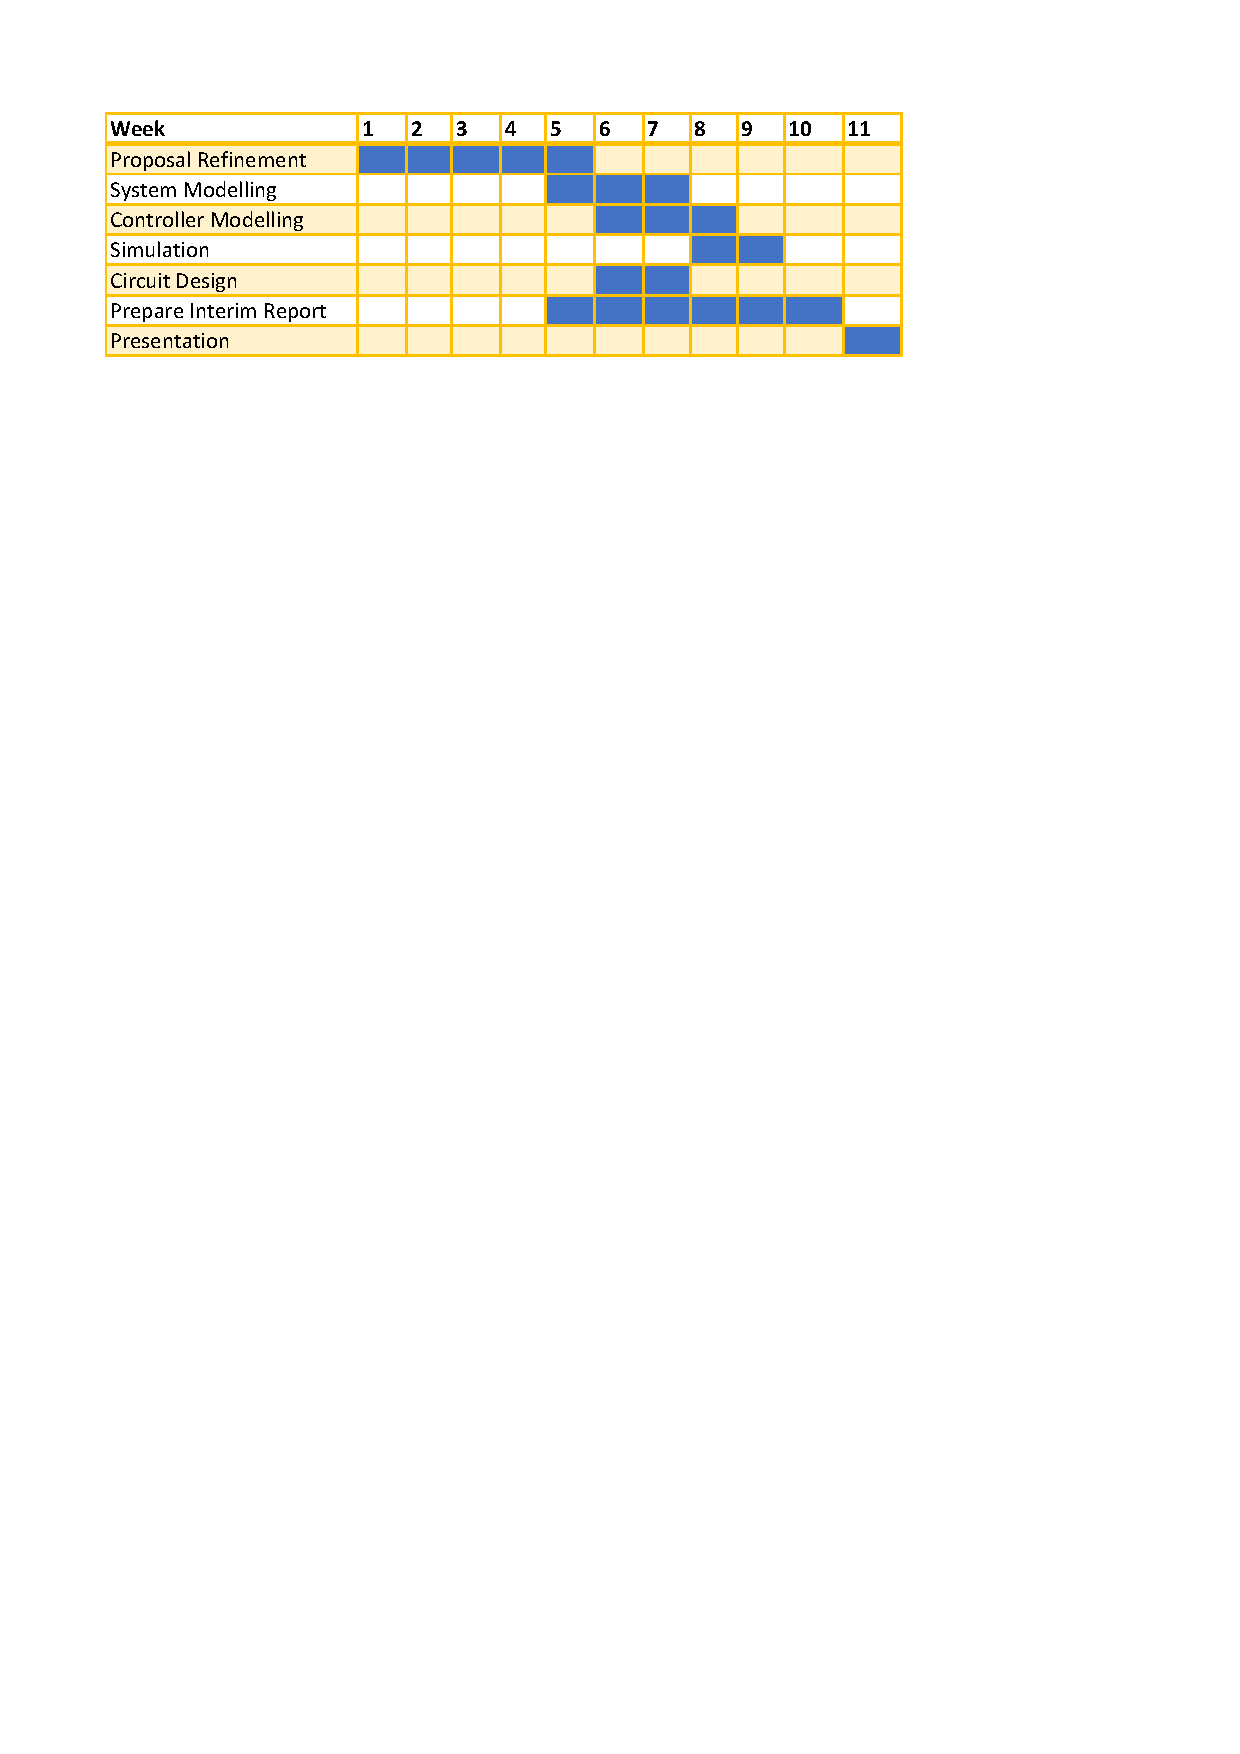
\includegraphics{Figures/workplan}
% 	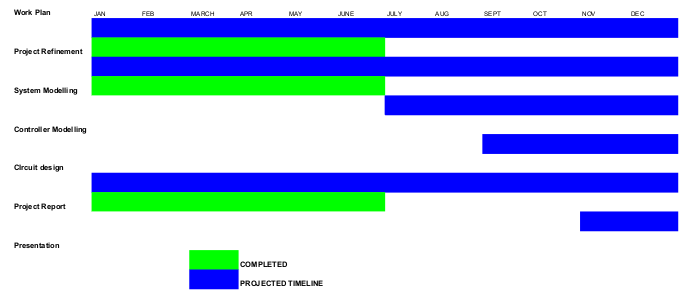
\includegraphics[width=1.059\linewidth]{Figures/project_wp}
% 	\caption{Work plan table}
% \end{figure}
